\chapter{Performance}
In this chapter, we will justify some choices that we made in the code that increase efficiency.
In the process, we will show and analyze the output of some optimization tools we used in order to test the performance of this library, as well as some of the aforementioned choices.

\section{Compiler flags}
When calling the \verb|g++| complier from the \verb|Makefile|, we used the following optimization flags, which instruct the compiler to maximize the code efficiency:
\begin{verbatim}
-march=native -O3 -msse2 -funroll-loops -ftree-vectorize
\end{verbatim}
In order to test their effects, we ran the \verb|maintest_nnws.cpp| test file using $n=10$ 5-dimensional data points, with and without the above flags, while timing both the algorithm execution and the density estimate with the help of the \verb|chrono| library.
The obtained average times (in TODO) were as follows:
\begin{center}
	\begin{tabular}{r|r|r|r}
	              	& \verb|run()| & \verb|eval_density()| & total \\ \hline
		without flags & 521762512 & 182770170 & 704532682 \\
		with flags    &  39615848 &  10353269 &  49969117 \\
		speedup       &       13x &       17x &       14x
	\end{tabular}
\end{center}
As one can see, the speedup resulting from the addition of these flags is very noticeable.


\section{In the \texttt{Algorithm} class}
One might note that the cluster cardinalities need not be part of the state, since they can be computed at any time from the allocations.
Despite that, we store the \verb|cardinalities| of the current iteration in a vector, which is first filled when the initial clusters are being built in the \verb|initialize()| function, then updated after the repositioning of each datum in \verb|sample_allocations()|.
This is because their explicit computation is needed in \verb|sample_allocations()| in order to be able to compute the masses of the current clusters.
The alternative is rebuilding the vector at each call of \verb|sample_allocations()|, which is $O(n)$; this is the same cost as the worst-case scenario of storing them externally, which can potentially happen in case 2.
In particular, if the first cluster is a singleton and the current datum moves from it to any other cluster, the whole vector must be shifted to the left by 1.
Therefore, the external storage is clearly a better choice. \\
A second point involves the usage of sparse Eigen matrices instead of dense ones in \verb|cluster_estimate()|.
It is mandatory to store the dissimilarity matrix for each of the $K$ iterations must be stored, so that the Frobenius norm of its difference with the mean dissimilarity can be computed.
These matrices add up to a total of $K n^2$ entries.
When the data size starts being moderately large, the memory usage becomes huge if using regular dense matrices.
On the contrary, the \verb|Eigen::SparseMatrix| class stores data points as a double vector of position and value, therefore greatly reducing the number of entries in the object, from $n^2$ to $2n$.
The dissimilarity matrices are indeed sparse objects, since their upper triangular part is never filled, and several of the entries in the lower triangular part may be zero as well.
In order to fill this type of matrix, a vector \verb|triplets_list| of \verb|Eigen::Triplet| objects must be used which stores each entry's position and value; the \verb|setFromTriplets()| method of the matrix is then used by passing \verb|triplets_list| as argument.
In order not to waste time reallocating massive amounts of data, a \verb|triplets_list.reserve()| call, and an estimate for the number of entries, are thus desirable.
Suppose that the $n$ data points are evenly distributed into $k$ clusters.
In such a case, the number of nonzero entries for the corresponding dissimilarity matrix (without the upper triangular part) is
$$ k \left(\binom{n/k}{2} - n\right) = \frac{n^2}{2k} -\frac{n}{2} - nk,$$
whilst the number for unbalanced clusters is slightly higher.
Therefore, $\frac{n^2}{4}$ is a good estimate for the number of entries.
This number is very close to the true amount if the number of clusters is small (e.g. $k=2,3,4$), which it often is. (Note that one could theoretically compute the exact number of nonzero entries of the dissimilarity matrix, but this would require additional computational costs which is not warranted for the size of a single vector.)
This relatively large amount of reserved space does not significantly impact the overall memory usage, since the \verb|triplets_list| vector is destroyed after each dissimilarity matrix is computed. \\
The usage of sparse matrices instead of dense ones does not hinder computational time either, since the Eigen library also heavily optimizes computations with sparse objects.
Nevertheless, an efficiency test was performed, this time using the Python interface, on the already implemented tests 1-6 (TODO?) with 500 algorithm iterations and 100 burn-in ones, using sparse matrices first and then the same operations but with dense matrices.
The results were as follows, again in TODO:
\begin{center}
	\begin{tabular}{c|c|c}
       &      sparse    &      dense     \\ \hline
test 1 & 4.51696840e+07 & 4.15315598e+07 \\
test 2 & 1.18633301e+09 & 9.17060859e+08 \\
test 3 & 2.91540577e+07 & 3.00693867e+07 \\
test 4 & 1.27339513e+08 & 1.22764857e+08 \\
test 5 & 1.50049441e+08 & 1.37240555e+08 \\
test 6 & 1.28818714e+08 & 1.16328396e+08
	\end{tabular}
\end{center}
As one can see, the performance is on average nearly identical for both types of implementation, with a difference of only less than 10\% for the multivariate tests 5 and 6 in favour of the dense case. \\
Finally, one more possible improvement for the current implementation is using a completely different approach of storing the data, e.g. with an \verb|std::map| in which each entry is a cluster that holds objects representing the data points themselves, instead of just storing the allocations labels.
This may be a way to erase and add clusters more efficiently.
Testing this assumption would be very difficult, since it would require implementing all data structures from scratch; nonetheless we think that using vectorial structures is more efficient for everything else, and therefore the correct choice.

\section{In the \texttt{Hierarchy} classes}
% NNW Stan likelihood, also with 5x data TODO



\section{Profiling analysis}
\verb|callgrind| is a command-line profiling tool that observes the running of the executable it is given as argument and records the call history among all functions that were called in it.
The output is then saved in a \verb|callgrind.out| file, which can be read with the use of the KCacheGrind GUI.
The following two commands were run, each on the C++ main test file for both the univariate case (with \verb|HierarchyNNIG<HypersFixedNNIG>|) and the multivariate case (with \verb|HierarchyNNW<HypersFixedNNW>|):
\begin{verbatim}
valgrind --tool=callgrind ./maintest_uni csv/data_uni.csv neal2 memory
valgrind --tool=callgrind ./maintest_multi csv/data_multi.csv neal2 memory
\end{verbatim}
The output of the univariate case produced the following dependence graph:
\begin{figure}[h]
	\centering
		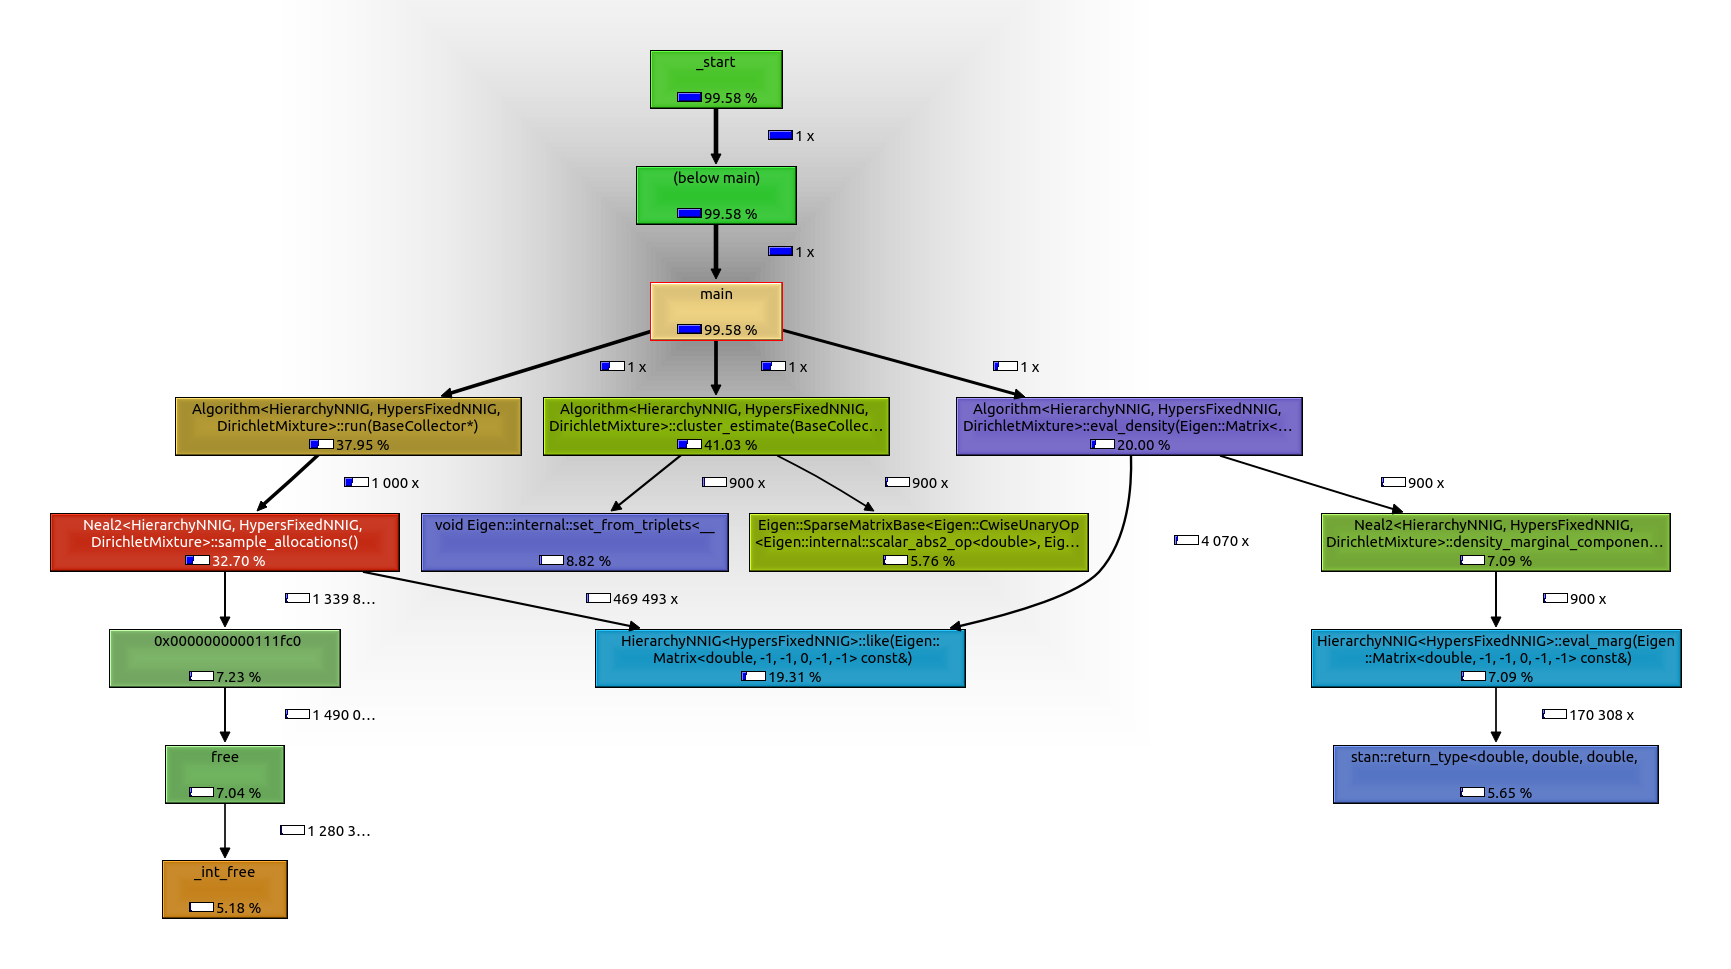
\includegraphics[scale=0.35]{etc/kcg_uni.png}
		%\captionsetup{labelformat=empty}
		%\caption{}
\end{figure}
blah blah blah TODO
\begin{figure}[h]
		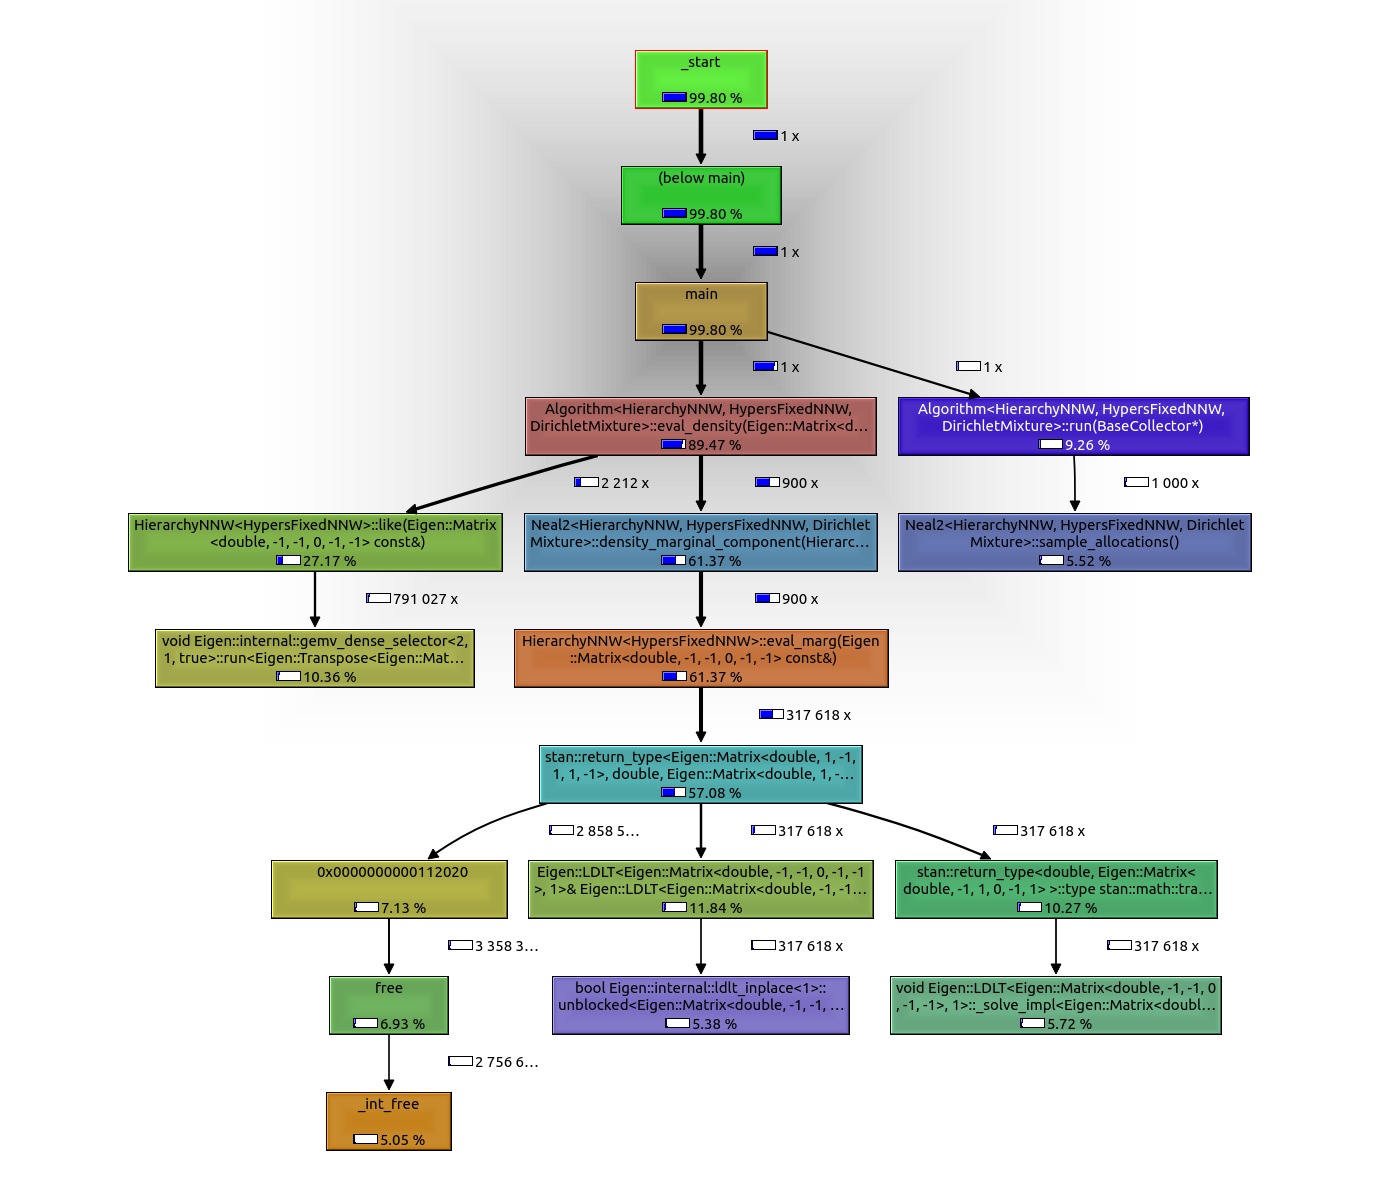
\includegraphics[scale=0.35]{etc/kcg_multi.png}
		%\captionsetup{labelformat=empty}
		%\caption{}
\end{figure}
